\documentclass[10pt,a4paper]{article}
\usepackage[a4paper,margin=17mm,headheight=15pt,footskip=13mm]{geometry}
\usepackage{fontspec}
\setmainfont{Noto Sans}
\setsansfont{Inter}
\setmonofont{DejaVu Sans Mono}[Scale=0.84]
\usepackage{amsmath,amssymb,mathtools}
\usepackage{microtype}
\usepackage{xcolor}
\usepackage{booktabs,longtable,tabularx,array,multirow,colortbl}
\usepackage{enumitem}
\usepackage{fancyhdr}
\usepackage{titlesec}
\usepackage{caption}
\usepackage{float}
\usepackage{graphicx}
\usepackage{tcolorbox}
\tcbuselibrary{breakable,skins}
\usepackage{fvextra}
\usepackage{hyperref}
\usepackage{bookmark}
\usepackage{lastpage}
\usepackage{ragged2e}
\usepackage{seqsplit}
\usepackage{pdflscape}

\definecolor{UGTSNavy}{HTML}{0D2B3A}
\definecolor{UGTSTeal}{HTML}{16979B}
\definecolor{UGTSGold}{HTML}{D4A21B}
\definecolor{UGTSCoral}{HTML}{CF6A5A}
\definecolor{UGTSPurple}{HTML}{6B5D96}
\definecolor{UGTSGreen}{HTML}{3F8D6A}
\definecolor{UGTSLight}{HTML}{EDF6F6}
\definecolor{UGTSLightGold}{HTML}{FBF5E4}
\definecolor{UGTSLightPurple}{HTML}{F2EFF8}
\definecolor{UGTSGrey}{HTML}{66737B}
\definecolor{UGTSDark}{HTML}{15252E}
\definecolor{UGTSRedLight}{HTML}{FAECE9}

\hypersetup{
  colorlinks=true,
  linkcolor=UGTSTeal,
  urlcolor=UGTSPurple,
  citecolor=UGTSTeal,
  pdftitle={UGTS-KC 3.6.2 SCLP - Swept-Cone Log-Polar Packing},
  pdfauthor={Tom Klootwijk (requester-supplied attribution)},
  pdfsubject={Formal integration of swept cone geometry, log-polar metric calculus, topology, grammar and finite 64-bit packing},
  pdfkeywords={UGTS, kinematic calculus, signed distance, cone, log-polar, Klein bottle, radix trie, Morton key, L-system, topology}
}

\pagestyle{fancy}
\fancyhf{}
\fancyhead[L]{\sffamily\small\color{UGTSNavy}\textbf{UGTS-KC 3.6.2 -- SCLP}}
\fancyhead[R]{\sffamily\small\color{UGTSGrey}Swept-Cone Log-Polar Packing}
\fancyfoot[L]{\sffamily\scriptsize\color{UGTSGrey}Tom Klootwijk -- requester-supplied attribution}
\fancyfoot[R]{\sffamily\scriptsize\color{UGTSGrey}Page \thepage\ of \pageref{LastPage}}
\renewcommand{\headrulewidth}{0.4pt}
\renewcommand{\footrulewidth}{0pt}

\titleformat{\section}{\sffamily\Large\bfseries\color{UGTSNavy}}{\thesection}{0.65em}{}
\titleformat{\subsection}{\sffamily\large\bfseries\color{UGTSTeal}}{\thesubsection}{0.55em}{}
\titleformat{\subsubsection}{\sffamily\normalsize\bfseries\color{UGTSPurple}}{\thesubsubsection}{0.5em}{}
\titlespacing*{\section}{0pt}{2.0ex plus .4ex minus .2ex}{0.8ex}
\titlespacing*{\subsection}{0pt}{1.5ex plus .3ex minus .2ex}{0.5ex}

\captionsetup{font=small,labelfont={bf,color=UGTSNavy},textfont={color=UGTSGrey},justification=centering}
\setlist[itemize]{leftmargin=1.5em,itemsep=0.25em,topsep=0.35em}
\setlist[enumerate]{leftmargin=1.7em,itemsep=0.3em,topsep=0.35em}
\setlength{\parindent}{0pt}
\setlength{\parskip}{0.50em}
\emergencystretch=2em

\newtcolorbox{decisionbox}[1][]{enhanced,breakable,colback=UGTSLight,colframe=UGTSTeal,boxrule=0.9pt,arc=1.8mm,left=2.5mm,right=2.5mm,top=1.7mm,bottom=1.7mm,fonttitle=\sffamily\bfseries,title=FORMAL DECISION,#1}
\newtcolorbox{definitionbox}[1][]{enhanced,breakable,colback=UGTSLightPurple,colframe=UGTSPurple,boxrule=0.8pt,arc=1.6mm,left=2.5mm,right=2.5mm,top=1.6mm,bottom=1.6mm,fonttitle=\sffamily\bfseries,title=FORMAL DEFINITION,#1}
\newtcolorbox{proofbox}[1][]{enhanced,breakable,colback=UGTSLightGold,colframe=UGTSGold,boxrule=0.8pt,arc=1.6mm,left=2.5mm,right=2.5mm,top=1.6mm,bottom=1.6mm,fonttitle=\sffamily\bfseries,title=DERIVATION / INVARIANT,#1}
\newtcolorbox{boundbox}[1][]{enhanced,breakable,colback=UGTSRedLight,colframe=UGTSCoral,boxrule=0.8pt,arc=1.6mm,left=2.5mm,right=2.5mm,top=1.6mm,bottom=1.6mm,fonttitle=\sffamily\bfseries,title=EVIDENCE BOUNDARY,#1}
\newtcolorbox{metricbox}[1][]{enhanced,breakable,colback=white,colframe=UGTSGreen,boxrule=0.8pt,arc=1.6mm,left=2.5mm,right=2.5mm,top=1.6mm,bottom=1.6mm,fonttitle=\sffamily\bfseries,title=EXACT METRICS,#1}

\newcommand{\code}[1]{\texttt{#1}}
\newcommand{\Sone}{\mathbb S^1}
\newcommand{\Ftwo}{\mathbb F_2}

\begin{document}
\pagenumbering{gobble}

\begin{titlepage}
\pagecolor{UGTSNavy}
\color{white}
\vspace*{9mm}
{\sffamily\bfseries\fontsize{34}{39}\selectfont UGTS-KC 3.6.2 -- SCLP\par}
\vspace{4mm}
{\sffamily\fontsize{21}{25}\selectfont Swept-Cone Log-Polar Packing\par}
\vspace{6mm}
{\sffamily\large Formal geometric-topological and kinematic delta over 3.6.1 BEA\par}
\vspace{12mm}

\begin{tcolorbox}[enhanced,colback=white,colframe=UGTSTeal,boxrule=1.2pt,arc=2mm,left=5mm,right=5mm,top=4mm,bottom=4mm]
\color{UGTSDark}
\textbf{Integrated source mechanisms}\par
A finite cone defined by slant length and half-angle; an exact cone signed-distance relation; a certified translational sweep bound; two local spherical supports; a log-polar chart with metric, Jacobian, velocity and acceleration calculus; a deterministic one-bit perturbation interval; time-to-phase winding; a source half-turn bundle twist and a separate reflective Klein quotient; a missing-shackle constraint-release certificate; a bounded binary L-system; distinct contiguous and Morton 64-bit keys; and an audited memory/complexity boundary.
\end{tcolorbox}

\vfill
{\sffamily\Large\bfseries Tom Klootwijk\par}
{\sffamily\large 10-07-1990 \quad NL200678942\par}
\vspace{3mm}
{\sffamily\small Requester-supplied attribution; identifiers not independently verified.\par}
\vspace{9mm}
{\sffamily\small Version 3.6.2 -- generated 17 August 2026\par}
{\sffamily\small The attached source is distilled without historical, dialect, renderer or physical-chaos escalation.\par}
\end{titlepage}
\nopagecolor
\color{UGTSDark}

\section*{Abstract}
The attached 13-page source collects a dense chain of motifs: a sweeping cone and sphere relations; analytical one-bit jitter; a log-encoded polar look-up space; lower-case $\phi$ as a hoop coordinate; angular ``change of change'' at a torque hinge; a missing shackle; a Klein-bottle-style wrap; time winding around an SDF-zero coil; bit shifts and binary bifurcation; a parametric L-system; instant state lookup; a 64-bit coordinate key; pointerless tree storage; and aggressive compression claims. The document also explicitly removes rasterization, ray marching and rendering from the intended core.

Version 3.6.2 converts those motifs into a finite referential substrate. It preserves the source terminology where technically meaningful, while separating overloaded symbols, coordinate effects, physical dynamics, topology, indexing and information loss. The resulting SCLP profile contains 50 atomic delta operators, 22 content-addressed definitions, a JSON Schema, two exact 64-bit key codecs, a dependency-free Python reference runtime, 70 new executable tests and the retained 83 tests from versions 3.6/3.6.1.

\begin{decisionbox}
The authoritative object is not an image, mesh, ray-marched volume or frame loop. It is a typed state-and-relation package that can answer geometric, topological, kinematic, branch, key and event queries. The output returns to the ordinary UGTS sequence: support $\rightarrow$ compatibility $\rightarrow$ guard $\rightarrow$ verified event $\rightarrow$ transition $\rightarrow$ lineage.
\end{decisionbox}

\tableofcontents
\clearpage
\pagenumbering{arabic}

\section{Source scope and extraction discipline}

\subsection{Registered source}
The immediate source is a 13-page exported dialogue whose first prompt combines a sweeping cone, one-bit jitter, the cone's triangular side and circular base, a sphere, a torque hinge, two spherical ``eyes'', a log-polar LUT, a Klein-bottle motif, a binary tree and lower-case $\phi$. Its later pages progressively remove the graphics interpretation and request a purely packed geometric-topological substrate, a formal grammar, instant state lookup, a 64-bit allocation and exact compression metrics.

\begin{Verbatim}[breaklines=true,fontsize=\small]
SHA-256: 7e29c1c800d905268f35084a6a4c7d9c1cfed50c926c63a8ec2c79021e32ab63
Pages: 13
Raw source redistributed in ZIP: no
\end{Verbatim}

The relevant page groups are:
\begin{itemize}
\item pages 1--3: finite-cone/SDF language, one-bit jitter, spheres, log-polar coordinates, local radial step and angular acceleration;
\item pages 3--5: time winding, chirality inversion, binary traversal and branch selection;
\item pages 6--8: a branch-conditioned L-system and a proposed instantaneous movement vector;
\item pages 9--11: explicit removal of rendering, a one-bit radix structure, a topological twist and a static typed state lookup;
\item pages 11--13: the 20/18/14/12 allocation, Morton-style interleaving, pointerless storage and width/compression claims.
\end{itemize}

\subsection{Admission rule}
A source motif enters the 3.6.2 core only if it becomes one of the following: a typed coordinate, a finite relation, a support, a metric/Jacobian, a transition/gluing map, a branch rule, a finite grammar, a content-addressed definition, a finite key codec, a measurable error bound or an explicit claims-ledger entry.

\begin{boundbox}
The source includes useful equations and also overstatements. Version 3.6.2 does not silently replace the source. It records both the source form and the normalized form. In particular, the source half-turn map is preserved as its own bundle profile; the actual orientation-reversing Klein profile is separate.
\end{boundbox}

\section{Canonical 3.6.2 architecture}

\begin{figure}[H]
\centering
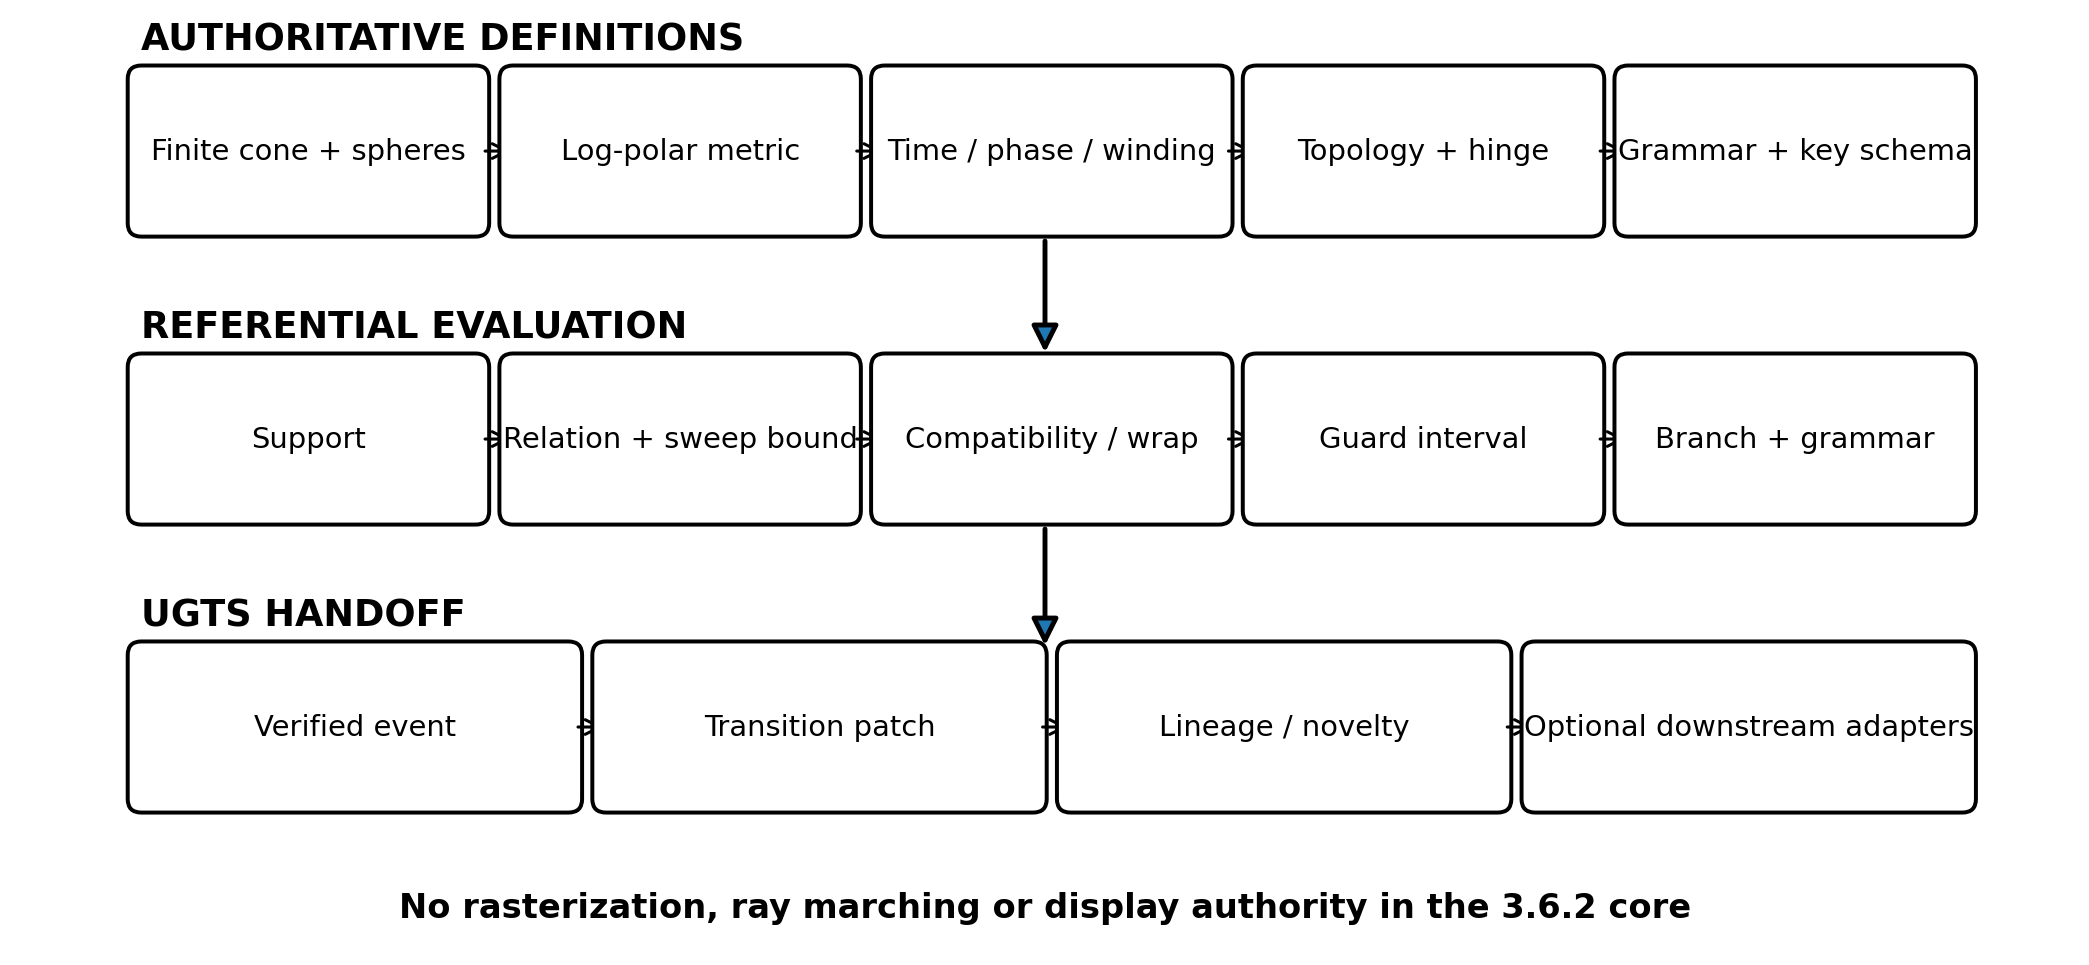
\includegraphics[width=\textwidth]{figures/sclp362_architecture.png}
\caption{SCLP definitions and evaluation remain upstream of the canonical UGTS event handoff.}
\end{figure}

The typed state is expanded to
\[
q=(x,t,\rho,\theta,\phi,\dot\phi,\ddot\phi,o,s,b,\omega_L,K,a,\mathcal L,u),
\]
where $x$ is position; $t$ is linear time; $(\rho,\theta)$ is a local chart; $\phi\in\Sone$ is the hoop/hinge angle; $o\in\{-1,+1\}$ is orientation; $s$ is a sheet; $b$ is a branch bit; $\omega_L$ is a finite grammar-state word; $K$ is a 64-bit address; $a$ is a generative address; $\mathcal L$ is lineage; and $u$ is uncertainty.

\subsection{Symbol contract}
The source overloads several symbols. SCLP imposes this non-negotiable contract:
\begin{center}
\begin{tabularx}{0.95\textwidth}{lX}
\toprule
\textbf{Symbol} & \textbf{Typed use}\\
\midrule
$T$ & cone slant length; never time, torque or a bit shift\\
$t$ & continuous linear time\\
$X$ & a declared modular tick or lookup-time coordinate\\
$\phi$ & periodic hinge/hoop angle in $\Sone$; not the golden ratio $\Phi$\\
$\Delta\rho$ & log-radius increment\\
$\Delta t$ & time increment\\
$\epsilon_j$ & bounded jitter amplitude\\
$\epsilon_g$ & event guard margin\\
$b$ & branch, predicate or jitter bit; never full state\\
\bottomrule
\end{tabularx}
\end{center}

\section{Finite cone, circle and sphere relations}

\subsection{Cone parameterization}
A side length alone does not determine a right circular cone. SCLP retains the source's side parameter $T$ and adds the required half-angle $\alpha$:
\[
h=T\cos\alpha,\qquad R=T\sin\alpha,
\]
with $T>0$ and $0<\alpha<\pi/2$. The circular base is the disk of radius $R$ in the plane $z=h$ relative to the apex/axis frame.

\begin{figure}[H]
\centering
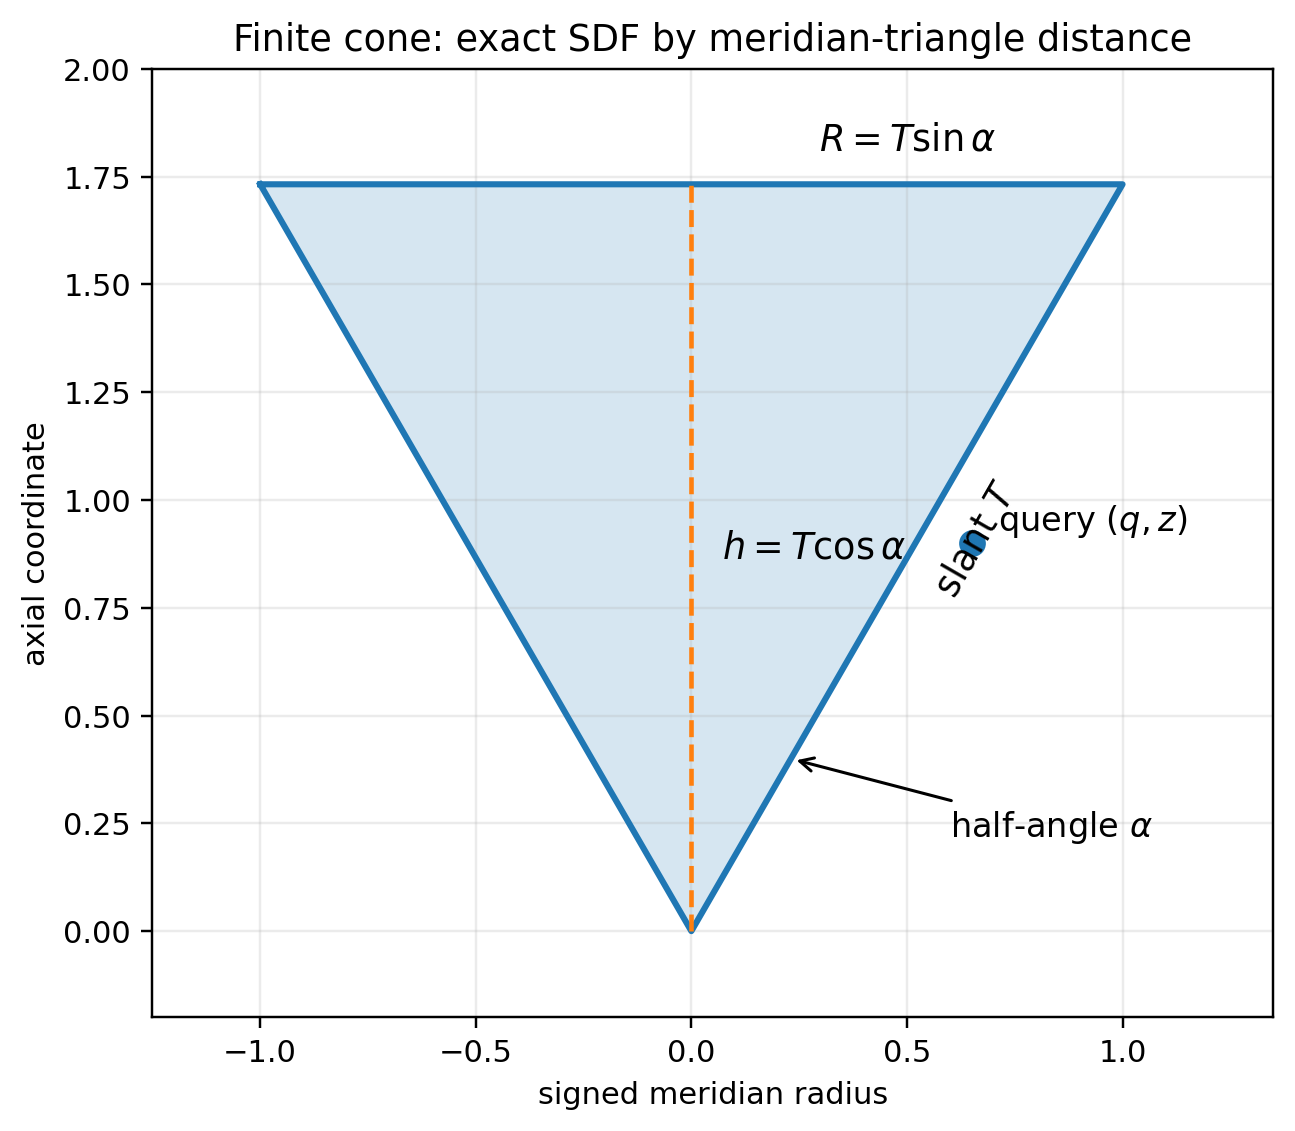
\includegraphics[width=0.68\textwidth]{figures/sclp362_cone_geometry.png}
\caption{The triangular side view and circular solid are joined by rotational symmetry.}
\end{figure}

For apex $c$, unit axis $a$ and query $x$, define
\[
z=a\cdot(x-c),\qquad q=\|(x-c)-za\|.
\]
The exact Euclidean signed distance is the signed distance from $(q,z)$ to the filled meridian triangle with vertices $(-R,h)$, $(R,h)$ and $(0,0)$. The sign is negative exactly when
\[
0\le z\le h,\qquad q\le z\tan\alpha.
\]

\subsection{Paired spherical support}
The source's ``two-sphered eye'' is normalized as two local sphere relations
\[
f_L(x)=\|x-c_L\|-R_L,\qquad f_R(x)=\|x-c_R\|-R_R.
\]
A profile chooses union, intersection or either-with-tag admission. The overlap flag is retained separately, so the two supports can function as a binocular pair, a dual sensor, two compatibility chambers or a local shared-domain test without a biological claim.

\section{Sweeping cone as a certified relation family}

Let $C$ be the finite cone and let $s(u)$ be a finite translation path for $u\in[0,1]$. The sweep relation is
\[
F_{\mathrm{sweep}}(x)=\inf_{u\in[0,1]} d_C(x-s(u)).
\]
For a linear segment of length $L$, $n\ge2$ uniform samples and sample minimum $m_n$, signed distance under translation is 1-Lipschitz. Therefore
\[
m_n-\frac{L}{2(n-1)}\le F_{\mathrm{sweep}}(x)\le m_n.
\]

\begin{proofbox}
The closest parameter $u^*$ lies no farther than $1/[2(n-1)]$ from some sample. Translating the cone by a spatial distance $\delta$ changes its signed distance at a fixed query by at most $\delta$. The interval follows. It becomes exact for a zero-length sweep and shrinks monotonically with sample density.
\end{proofbox}

The reference instance uses $L=0.75$, $n=65$ and yields
\[
-0.3024764633\le F_{\mathrm{sweep}}\le-0.2966170883,
\]
so the query has a certified interior witness under a 0.001 guard band.

\begin{boundbox}
This is not a universal closed-form SDF for every swept, rotated or grammar-generated cone. The exact primitive SDF and the sweep interval are different typed objects. Rotating sweeps require an additional angular-speed/bounding-radius error term or a specialized solver.
\end{boundbox}

\section{Log-polar metric and kinematic calculus}

\subsection{Coordinate chart and explicit core}
The chart is
\[
\rho=\ln(r/r_0),\qquad \theta=\operatorname{atan2}(y,x),\qquad r=r_0e^\rho.
\]
The origin remains singular. Every profile therefore declares a core radius and returns a core flag instead of pretending that the logarithm removes $r=0$.

\begin{figure}[H]
\centering
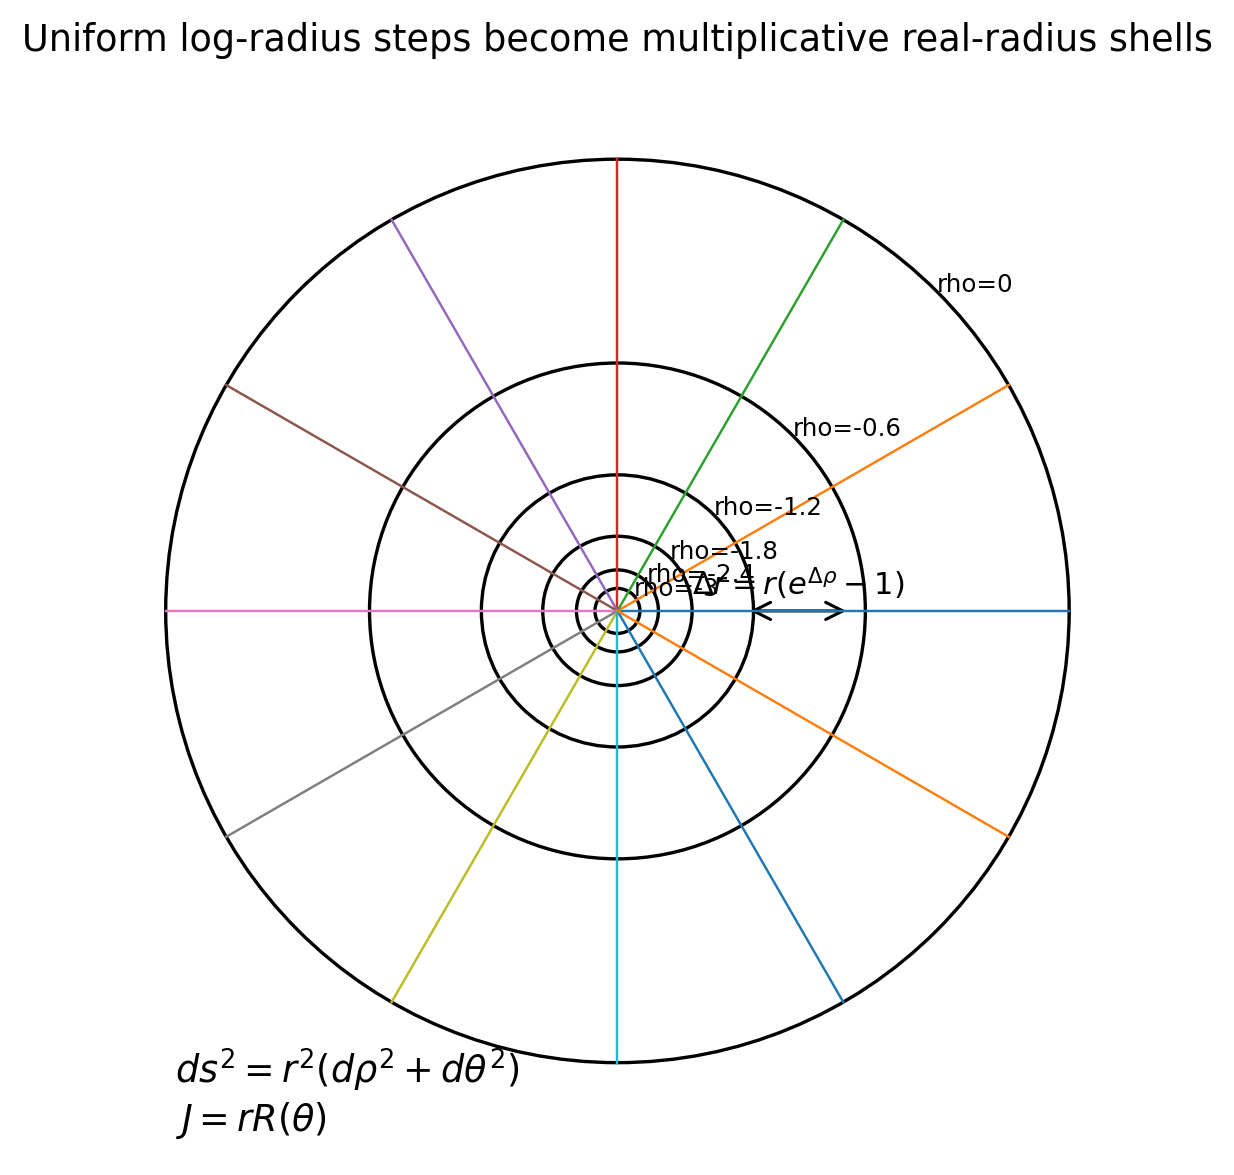
\includegraphics[width=0.72\textwidth]{figures/sclp362_logpolar_metric.png}
\caption{The log chart is a non-uniform coordinate representation, not infinite precision.}
\end{figure}

\subsection{Metric and exact local step}
The planar metric is conformal:
\[
ds^2=r^2(d\rho^2+d\theta^2),\qquad g(\rho)=r^2 I_2.
\]
A finite log step gives the exact real-radius increment
\[
\Delta r=r(e^{\Delta\rho}-1),
\]
not merely $r\Delta\rho$ except to first order.

\subsection{Jacobian, velocity and change of change}
The Jacobian is
\[
J=r\begin{bmatrix}
\cos\theta&-\sin\theta\\
\sin\theta&\cos\theta
\end{bmatrix}.
\]
With radial and angular unit vectors $e_r,e_\theta$,
\[
v=r(\dot\rho e_r+\dot\theta e_\theta),
\]
\[
a=r[(\ddot\rho+\dot\rho^2-\dot\theta^2)e_r+(\ddot\theta+2\dot\rho\dot\theta)e_\theta].
\]
This is the exact normalized meaning of ``change of change'' in the chart. If a scalar field has chart derivatives $(f_\rho,f_\theta)$, then
\[
\nabla_{xy}f=\frac{f_\rho e_r+f_\theta e_\theta}{r}.
\]
A coordinate component may scale as $e^{-\rho}$, but a physical force does not automatically do so: force requires a declared mechanics model and tensor transformation.

\section{One-bit jitter and guard intervals}

The source uses a one-bit analytical jitter as a high-frequency perturbation and as tree metadata. SCLP separates these roles. For seed, address $K$ and tick $X$,
\[
b=H(\text{seed},K,X)\bmod 2,\qquad \sigma=2b-1.
\]
An optional field perturbation is
\[
f_j=f+\epsilon_j\sigma.
\]
The authoritative relation is not discarded. Instead it receives the interval certificate
\[
f\in[f_j-\epsilon_j,f_j+\epsilon_j]
       =[f-\epsilon_j,f+\epsilon_j].
\]
The jitter profile is admissible only when $\epsilon_j<\epsilon_g$ and the interval cannot change the verified event class or ordering.

For the bundled example,
\begin{align*}
f&=-0.1700961894,\\
\epsilon_j&=10^{-4},\qquad \epsilon_g=10^{-3},\\
[f-\epsilon_j,f+\epsilon_j]&=[-0.1701961894,-0.1699961894].
\end{align*}
The entire interval remains negative, so the one-bit modulation cannot move this query across the zero relation.

\section{Time thread, phase and winding}

The source turns the 18:55 statement into a phase seed and a loop count. SCLP keeps the useful idea but not the claim that time itself stops being linear. Given reference tick $X_0$, period $P$ and linear tick $X$,
\[
u=\frac{X-X_0}{P},\qquad w=\lfloor u\rfloor,\qquad \psi=u-w\in[0,1).
\]
Here $\psi$ is the phase on $\Sone$ and $w$ is the winding lineage. The reference profile declares 18:55 as 1,135 minutes from midnight; that unit is metadata, not a universal constant.

At $X=1920$ and $P=256$, the example produces
\[
w=3,\qquad \psi=0.06640625,\qquad w\bmod2=1.
\]
Repeated phase coordinates therefore remain distinguishable by winding and lineage.

\section{Topological wrapping: source form and Klein form}

\begin{figure}[H]
\centering
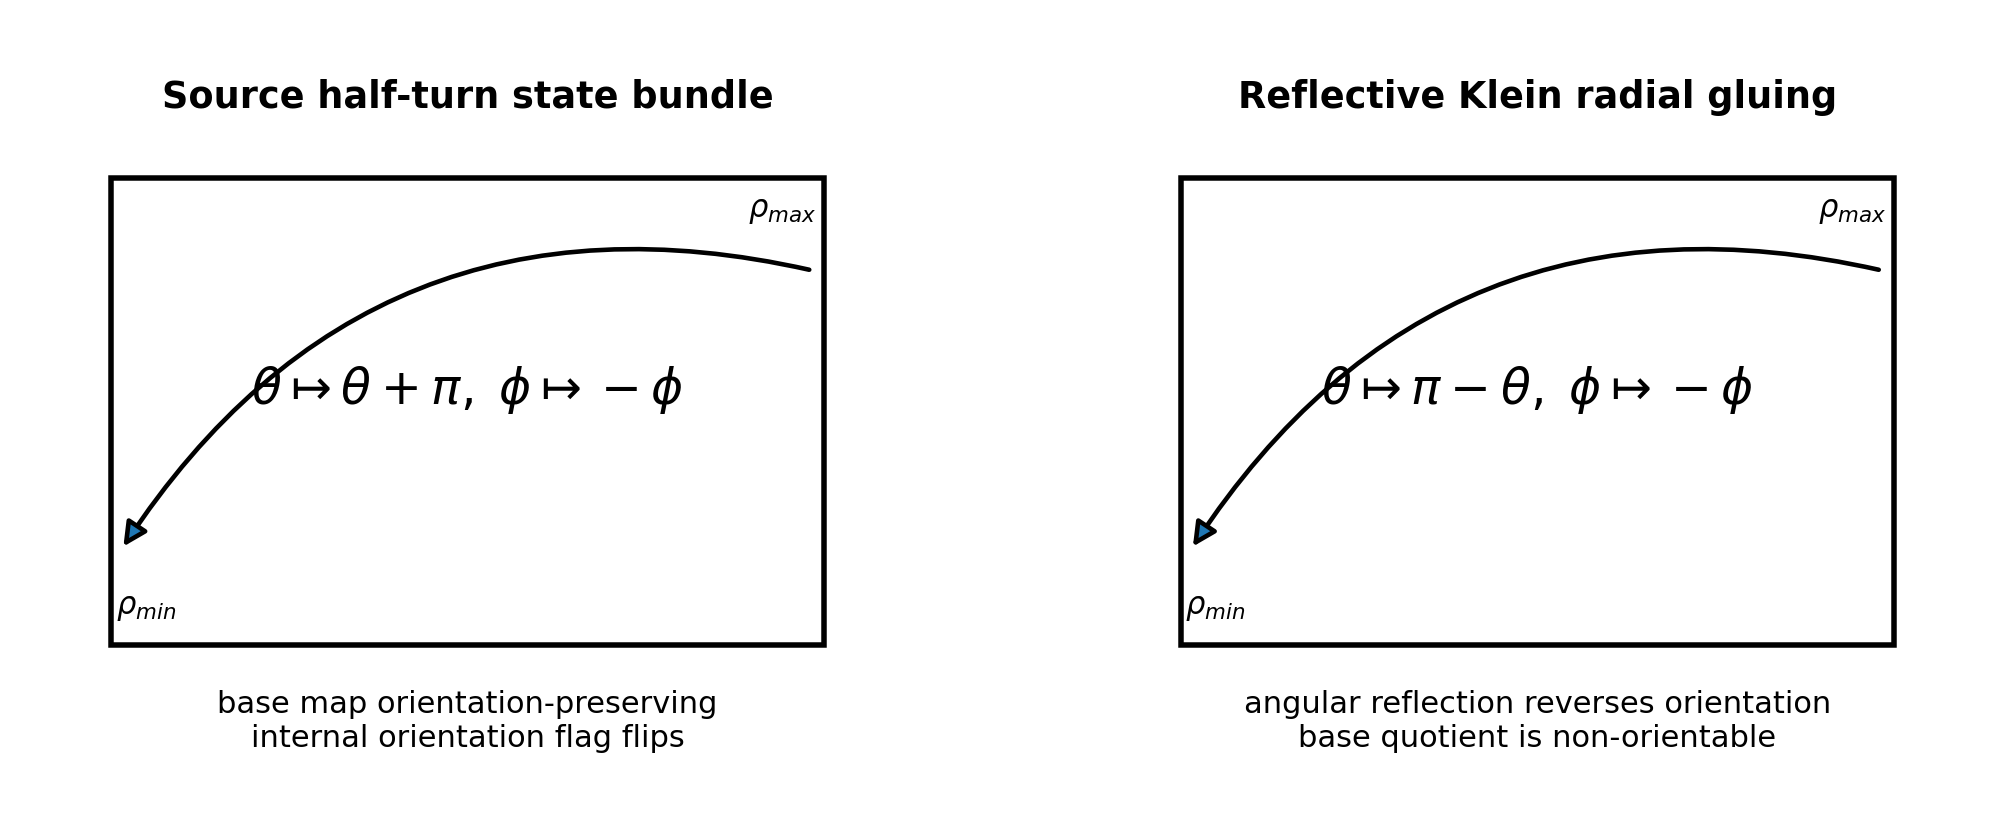
\includegraphics[width=0.92\textwidth]{figures/sclp362_topology_profiles.png}
\caption{The source half-turn formula and the orientation-reversing quotient are represented as separate profiles.}
\end{figure}

\subsection{Source half-turn bundle}
On an odd radial wrap, the literal source formula is retained as
\[
(\rho,\theta,\phi,o)\mapsto(\rho',\theta+\pi,-\phi,-o).
\]
Because $\theta\mapsto\theta+\pi$ is a rotation of the angular circle, it does not by itself make the base coordinate quotient non-orientable. The internal hoop/orientation state does flip, so the operation is useful as a twisted state bundle.

\subsection{Reflective Klein profile}
The actual non-orientable profile uses
\[
(\rho,\theta,\phi,o)\mapsto(\rho',\pi-\theta,-\phi,-o)
\]
on odd radial wraps, with periodic angular closure on the other boundary. The angular reflection has derivative $-1$, so the base gluing reverses orientation. The hoop coordinate and orientation flag flip with it.

For the shipped wrap example, $\rho=0.25$ in the interval $[-20,0)$ creates one wrap and returns
\[
\rho'=-19.75,\quad \theta'=-\pi,\quad \phi'=-0.34906585,\quad o'=-1.
\]
The chart transition changes coordinate components; it is not an instantaneous physical torque impulse.

\section{Hinge calculus and the missing shackle}

\subsection{Typed hinge state}
The hinge state is
\[
h=(\phi,\omega,\alpha)=(\phi,\dot\phi,\ddot\phi).
\]
Torque is not another name for angular acceleration. Only after a mechanical profile supplies inertia $I$, damping $c$ and stiffness $k$ may one compute, for example,
\[
\tau=I\alpha+c\omega+k\phi.
\]
The reflective chart map sends $(\phi,\omega,\alpha)$ to $(-\phi,-\omega,-\alpha)$ under the symmetric model.

\subsection{Constraint release}
Let a velocity constraint be
\[
A(q)\dot q=0.
\]
The missing shackle is represented by removing one declared row to obtain $A'$. The exact freedom gain is
\[
\Delta d=\operatorname{nullity}(A')-\operatorname{nullity}(A).
\]
In the reference matrix
\[
A=\begin{bmatrix}1&0&0\\0&1&0\end{bmatrix},
\]
removing the second row changes rank from 2 to 1 and nullity from 1 to 2, so $\Delta d=1$. This establishes an additional legal velocity direction. It does not establish chaos, a force law or a floating-base trajectory without further dynamics.

\subsection{Motion constrained to an SDF-zero coil}
For a regular zero surface $f(x)=0$ with unit normal $n$, a proposed velocity $v$ can be kept tangent to first order by
\[
P_T=I-nn^T,\qquad v_T=P_Tv,
\]
which guarantees $n\cdot v_T=0$. Numerical drift still requires projection or constrained integration.

\section{Bit branch, bifurcation and bounded L-system}

A branch guard returns $b\in\{0,1\}$ and selects a declared transition or production. A binary branch is not automatically a chaotic bifurcation. Chaos requires a specific dynamical map and evidence such as sensitivity or a positive Lyapunov exponent.

The reference parametric grammar rewrites each forward symbol $F(T)$ into two dyadically scaled branches with a signed turn, a balanced push/pop pair and a metric-aware jitter token. In schematic form,
\[
F(T)\Rightarrow F(T/2)\,[\,\pm\phi\;F(T/2)\,]J(\Delta r).
\]
The sign is selected by the branch bit and then multiplied by topological chirality. The automorphism $+\leftrightarrow-$ implements the source's turn reversal at the reflective boundary.

\begin{figure}[H]
\centering
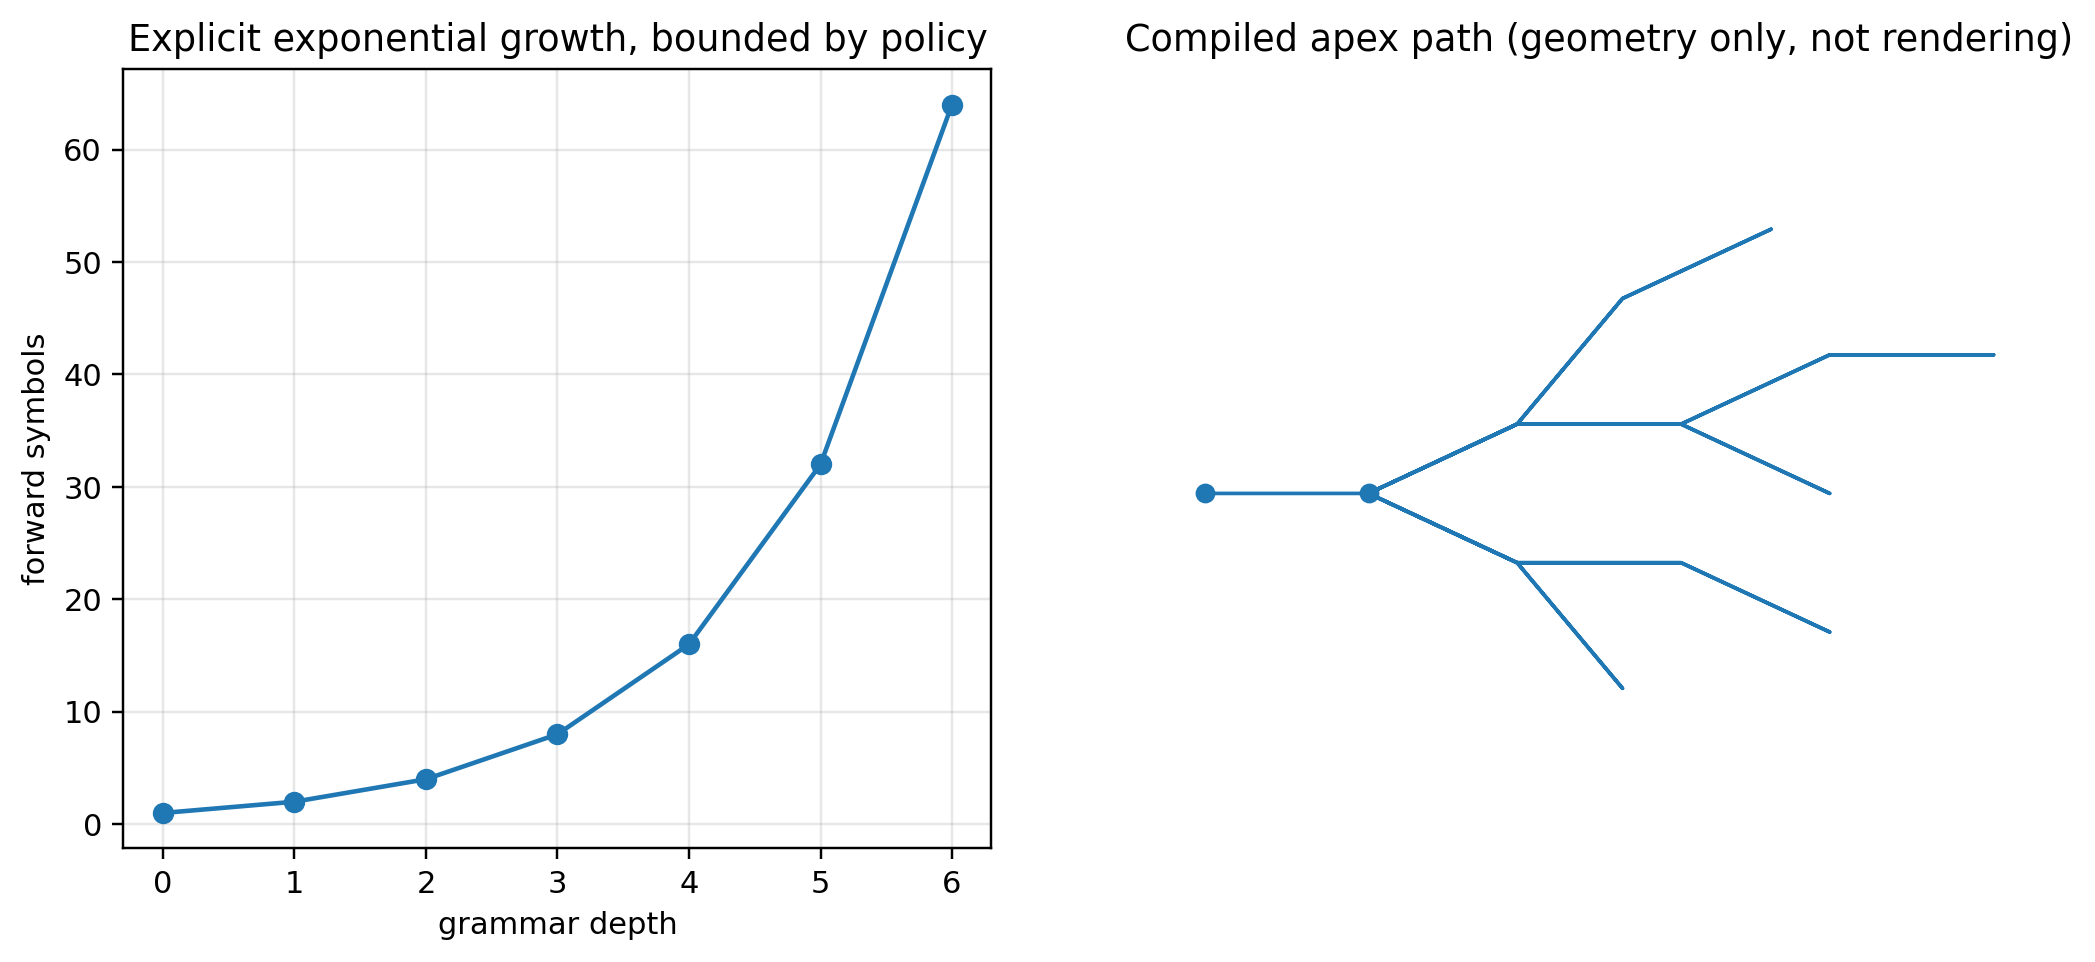
\includegraphics[width=0.88\textwidth]{figures/sclp362_grammar_growth.png}
\caption{Grammar growth is explicit, finite and budgeted; the compiled line is an apex path, not a rendered scene.}
\end{figure}

The example depth is 4. It produces 16 forward symbols, 76 total symbols, maximum stack depth 4 and a 12-bit grammar-state word of 1058. The implementation rejects depth, symbol or stack overflow.

\section{Bit shift as radix-trie refinement}

The source says a left shift moves deeper into a 1-bit binary search tree and halves log-radius/angle. SCLP corrects the mechanism:
\begin{itemize}
\item the structure is a radix-2 trie over fixed-width key prefixes, not a comparison-based BST;
\item appending a bit performs $p'=(p\ll1)\,|\,b$;
\item that bit fixes one scheduled coordinate bit in the Morton profile;
\item the corresponding integer cell interval is refined; decoded physical coordinates are not directly divided by two.
\end{itemize}

A 64-level path is therefore a sequence of coordinate refinements. Prefix bounds are executable: after each appended bit, no field interval can widen, and at least the scheduled field narrows.

\section{Two exact 64-bit key layouts}

The source page 12 simultaneously supplies contiguous bit ranges and a Morton-style interleaving equation. Those are not the same layout. Version 3.6.2 keeps both under separate IDs.

\begin{table}[H]
\centering
\small
\begin{tabularx}{0.96\textwidth}{lrrlX}
\toprule
\textbf{Field} & \textbf{Bits} & \textbf{States} & \textbf{Contiguous range} & \textbf{Quantization}\\
\midrule
rho & 20 & 1,048,576 & 63:44 & [-20,0]; step 1.9073504518e-05\\
theta & 18 & 262,144 & 43:26 & [0,2pi); step 2.39684498107e-05\\
time & 14 & 16,384 & 25:12 & modular ticks; step 1\\
phi & 12 & 4,096 & 11:0 & [0,2pi); step 0.00153398078789\\
\bottomrule
\end{tabularx}
\caption{Exact field widths for the 64-bit SCLP key.}
\end{table}


\begin{figure}[H]
\centering
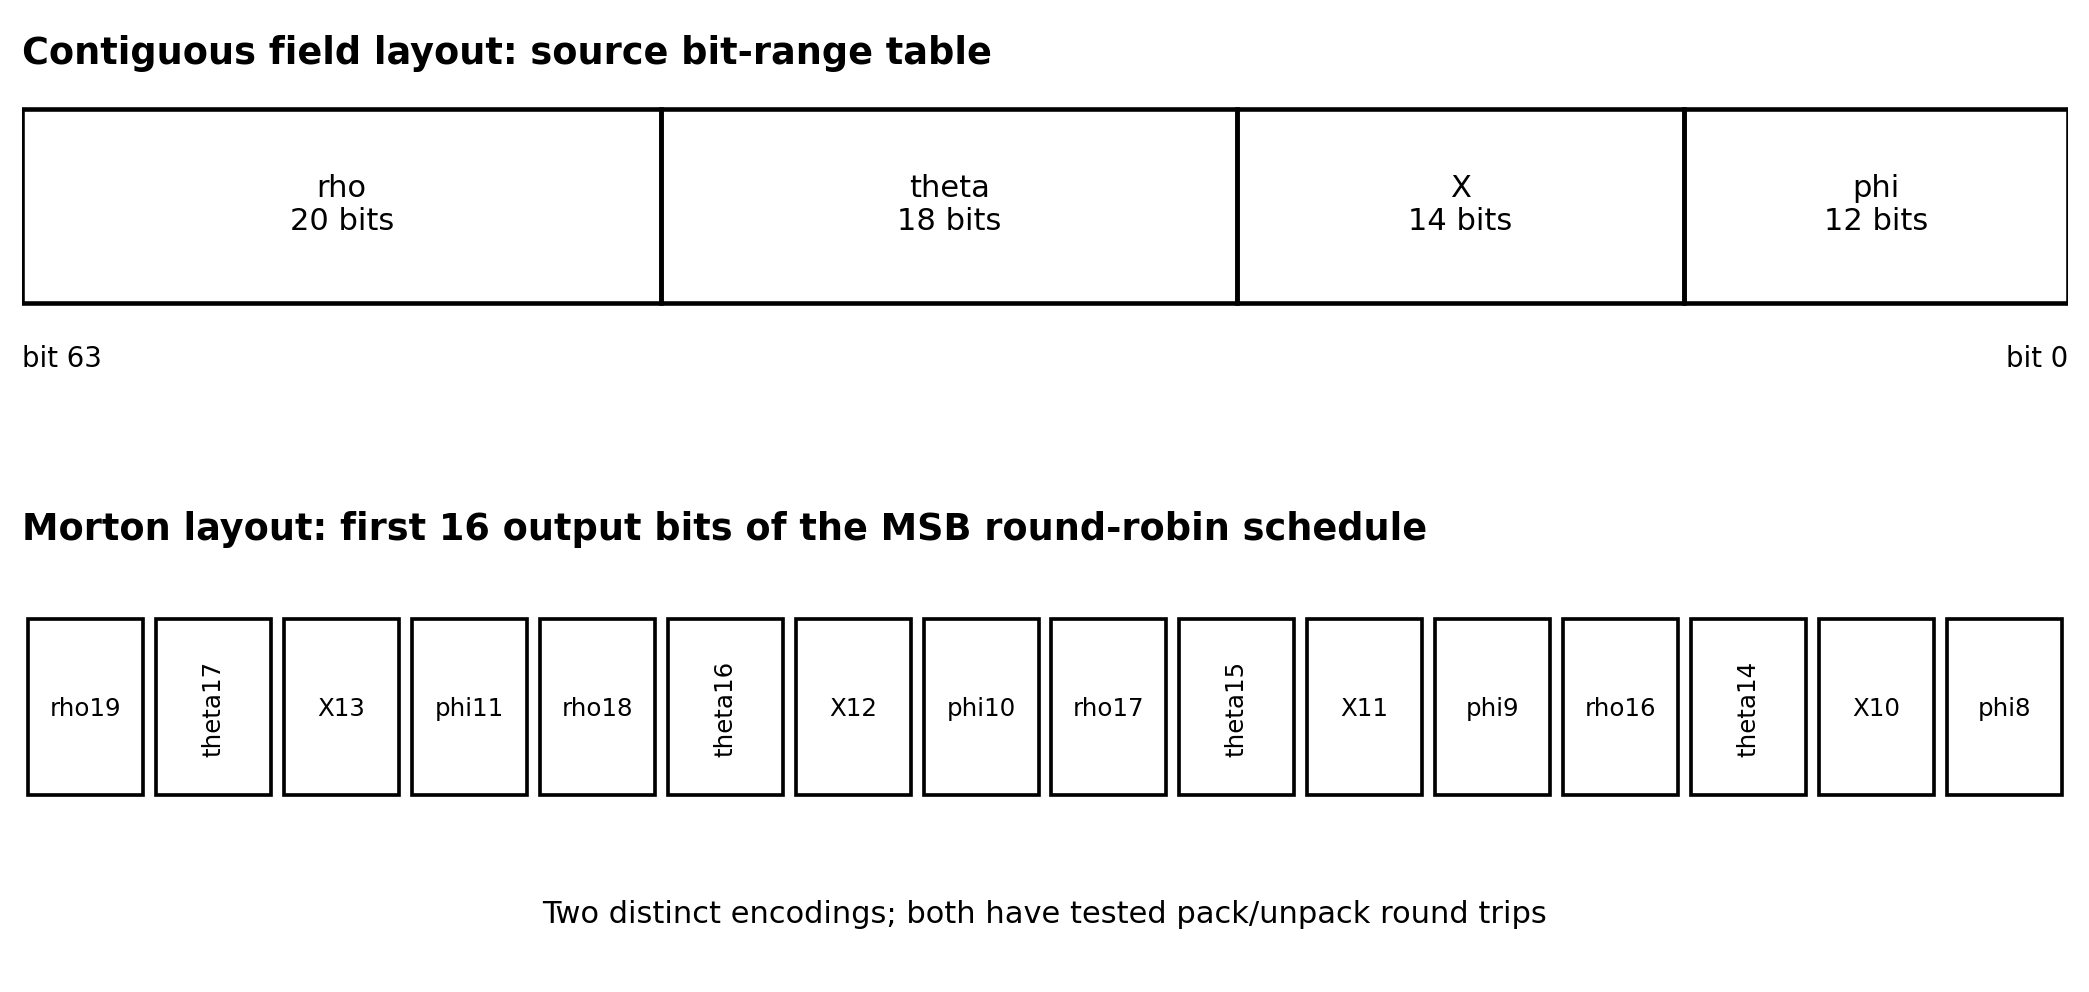
\includegraphics[width=0.94\textwidth]{figures/sclp362_key_layouts.png}
\caption{The key layouts are distinct and have independent pack/unpack tests.}
\end{figure}

The contiguous word is
\[
K_C=(q_\rho\ll44)\;|\;(q_\theta\ll26)\;|\;(q_X\ll12)\;|\;q_\phi.
\]
The Morton word consumes bits in MSB round-robin order:
\[
\rho_{19},\theta_{17},X_{13},\phi_{11},\rho_{18},\theta_{16},X_{12},\phi_{10},\ldots
\]
until all 64 source bits are used. The complete schedule is included as CSV and JSON.

For the reference state,
\begin{align*}
(q_\rho,q_\theta,q_X,q_\phi)&=(949111,0,1920,227),\\
K_C&=\code{0xe7b77000007800e3},\\
K_M&=\code{0x88823bb88099128b}.
\end{align*}
Both decode exactly to the same quantized tuple, while the words are intentionally different.

\begin{metricbox}
The finite address capacity is exactly
\[
2^{20}2^{18}2^{14}2^{12}=2^{64}=18,446,744,073,709,551,616.
\]
For $\rho\in[-20,0]$, the reference steps are $1.90735045\times10^{-5}$ in $\rho$, $2.39684498\times10^{-5}$ radians in $\theta$, 16,384 modular time states and $1.53398079\times10^{-3}$ radians in $\phi$.
\end{metricbox}

\section{Pointerless storage and compression audit}

A dense complete binary heap can infer children $2i+1$ and $2i+2$ without pointers. A sparse tree cannot simply prune arbitrary gaps and keep that formula without either reserving the gaps or adding topology/presence information. A succinct production structure needs a topology bitvector, a payload bitvector and rank/select or equivalent navigation metadata.

\begin{figure}[H]
\centering
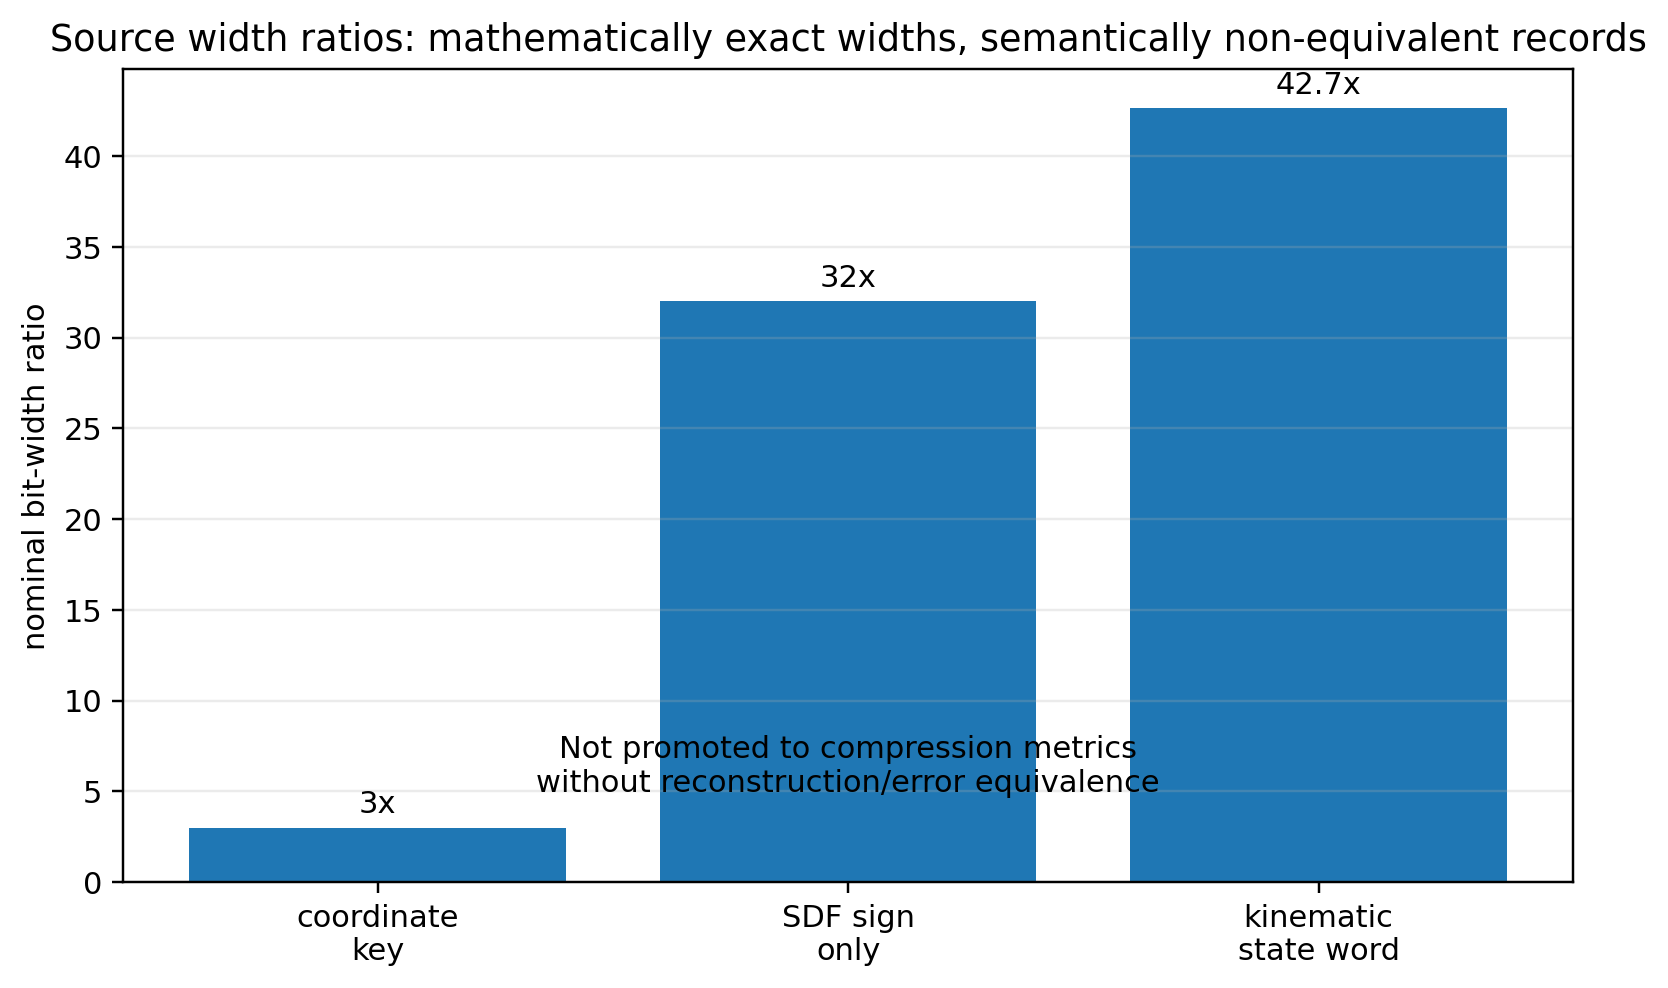
\includegraphics[width=0.72\textwidth]{figures/sclp362_compression_audit.png}
\caption{The source numbers are retained as width ratios and not promoted to equal-information compression.}
\end{figure}

The exact arithmetic is:
\[
192/64=3,
\qquad 32/1=32,
\qquad 512/12=42.666\overline6.
\]
But the compared records are not semantically equivalent:
\begin{itemize}
\item six float32 boundaries contain different information and error semantics from one quantized key;
\item a one-bit sign does not retain SDF magnitude, exact zero state or uncertainty;
\item a 12-bit state word can select only a finite versioned codebook, not encode an arbitrary $4\times4$ float matrix.
\end{itemize}
Eight raw 64-bit keys fit in a 64-byte cache line. This establishes capacity only, not eight evaluations in one cycle. The 64-bit profile is finite; it does not store infinite detail.

\section{Literal referential substrate integration}

The machine-readable example contains 22 content-addressed definitions. Each definition records ID, kind, domain, codomain, evaluation phase, dependencies, parameters, invariants, provenance and canonical SHA-256 content hash. Dependency ordering is acyclic and validated before execution.

The reference pipeline is:
\begin{enumerate}
\item select SCLP profile and typed symbol contract;
\item construct the finite cone and evaluate its exact relation;
\item test the paired-sphere support;
\item compute log-polar state, metric and phase/winding;
\item quantize and encode both 64-bit layouts;
\item refine a radix prefix and certify jitter;
\item evaluate source-twist and reflective-Klein profiles separately;
\item release the selected constraint row and evaluate hinge mechanics;
\item select the branch, expand the bounded grammar and certify the sweep;
\item audit width/memory claims;
\item issue an integrated certificate and hand off to UGTS.
\end{enumerate}

\begin{figure}[H]
\centering
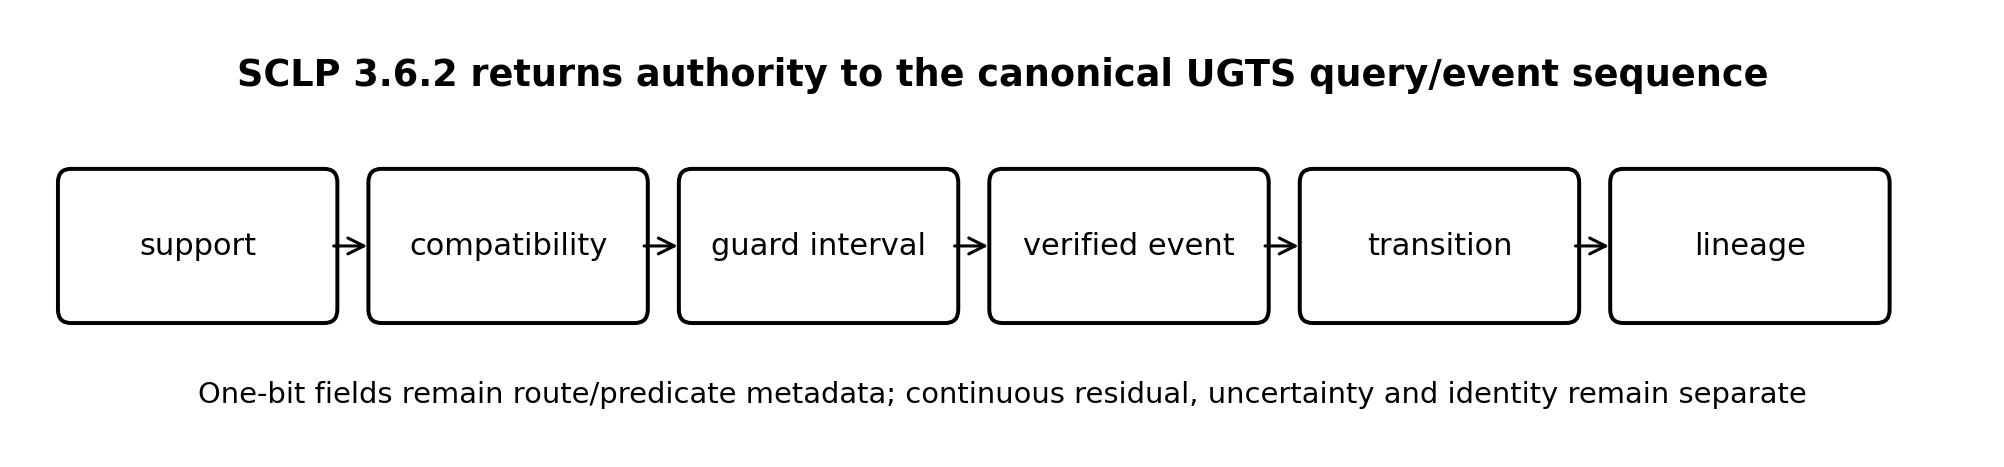
\includegraphics[width=0.94\textwidth]{figures/sclp362_event_handoff.png}
\caption{The new mechanisms do not replace the canonical event sequence.}
\end{figure}

The exact reference certificate is valid. Its notable fields are:
\begin{center}
\begin{tabularx}{0.95\textwidth}{lX}
\toprule
\textbf{Field} & \textbf{Result}\\
\midrule
cone residual & $-0.1700961894$ (interior)\\
log-polar state & $\rho=-1.8971199849$, $\theta=0$, metric scale $0.0225$\\
jitter interval & $[-0.1701961894,-0.1699961894]$, safe under 0.001 margin\\
time & phase $0.06640625$, winding 3\\
Klein wrap & one wrap, orientation $-1$, $\rho'=-19.75$\\
missing shackle & nullity $1\rightarrow2$, freedom gain 1\\
grammar & depth 4, 16 forward symbols, 76 total, state word 1058\\
sweep & certified interval $[-0.3024764633,-0.2966170883]$\\
key layouts & exact round trip for both; distinct words\\
\bottomrule
\end{tabularx}
\end{center}

\section{Reference implementation and verification}

The package retains all 3.6 and course-corrected 3.6.1 files and adds:
\begin{itemize}
\item \code{src/ugts36/sclp362.py}: geometry, metric, topology, constraints, grammar, key and metric operators;
\item \code{src/ugts36/sclp\_runtime.py}: literal referential pipeline evaluator;
\item \code{spec/SCLP\_3\_6\_2\_FORMAL\_DEFINITION.md};
\item a 50-operator CSV/JSON catalog and 20-entry claims ledger;
\item JSON Schema and content-addressed example substrate;
\item exact key-layout and 64-row Morton schedule files;
\item deterministic certificate, trace and demonstration;
\item editable LaTeX source, figures, tests, validation report and SHA-256 manifest.
\end{itemize}

The 70 new tests cover exact cone geometry, paired spheres, sweep intervals, log-polar derivatives, jitter bounds, time/winding, both topology profiles, hinge mechanics, constraint rank/nullity, tangent projection, finite grammar budgets, both key codecs, prefix refinement, trie accounting, metric qualifications, JSON Schema, content hashes, pipeline ordering and requester attribution.

Together with the retained 83 tests, the combined package contains 153 passing tests. These establish internal consistency and executable bounds. They do not validate a physical device, a universal performance advantage or a claim of infinite detail.

\section{Claims ledger and kill criteria}

\input{sclp362_claims_ledger_table.tex}

The 3.6.2 delta is rejected or simplified for a target application if any of the following occurs:
\begin{itemize}
\item quantization or jitter exceeds the event guard margin or changes event ordering;
\item the sweep interval remains too wide to classify the relation at the required tolerance;
\item grammar growth or branch density exceeds the declared budget;
\item key collisions, table occupancy or sparse-tree metadata erase the expected storage gain;
\item the source half-turn profile is incorrectly treated as a Klein base quotient;
\item the 12-bit grammar/state word cannot reconstruct the required state family;
\item pointerless layout, decoding or verification costs exceed a conventional index at equal error;
\item any width ratio is reported as compression without semantic and reconstruction equivalence;
\item a physical torque, force, chaos or throughput claim is made without a specified model and measurement.
\end{itemize}

\section{Final definition}

\begin{definitionbox}
UGTS-KC 3.6.2 SCLP is a finite, content-addressed, query-first delta in which a finite cone and paired spherical supports provide exact primitive relations; a translational sweep has a certified relation interval; a log-polar chart supplies a metric and kinematic calculus; one-bit jitter is bounded by an explicit guard interval; linear time maps to phase plus winding; topological wrapping is split into a literal half-turn bundle and a reflective Klein quotient; hinge and missing-shackle behavior are typed by angular state and constraint rank; branch bits drive a finite budgeted grammar; and 20/18/14/12 quantized fields are encoded by two explicit, invertible 64-bit layouts. Every result is passed to support, compatibility, guard, event, transition and lineage rather than to a renderer.
\end{definitionbox}

\begin{boundbox}
This document does not assert that the source's entire combined apparatus is a previously established physical theory. It provides a clean formal profile in which the recoverable geometric, topological, kinematic and packing mechanisms are explicit, testable and falsifiable.
\end{boundbox}

\clearpage
\appendix
\section{Complete SCLP 3.6.2 operator catalog}
\begin{landscape}
\scriptsize
\setlength{\tabcolsep}{2.5pt}
\renewcommand{\arraystretch}{1.14}
\begin{longtable}{p{0.19\linewidth} p{0.08\linewidth} p{0.15\linewidth} p{0.37\linewidth} p{0.10\linewidth} p{0.07\linewidth}}
\caption{Complete 50-operator SCLP 3.6.2 delta catalog.}\label{tab:sclp-ops}\\
\toprule
\textbf{Operator ID} & \textbf{Domain} & \textbf{Mechanism} & \textbf{Normalized technical definition} & \textbf{Disposition} & \textbf{Source}\\
\midrule
\endfirsthead
\toprule
\textbf{Operator ID} & \textbf{Domain} & \textbf{Mechanism} & \textbf{Normalized technical definition} & \textbf{Disposition} & \textbf{Source}\\
\midrule
\endhead
\texttt{sclp362.profile.packed-swept-cone-v1} & Profile & Packed SCLP profile & Typed finite profile combining a cone relation, log-polar chart, modular time, topology, grammar and two 64-bit key layouts. & ENGINEERING-DERIVED & pp.9-13\\
\texttt{sclp362.type.symbol-separation-v1} & Typing & Overloaded-symbol separation & T is slant length; t is linear time; X is a modular tick; phi is a hoop angle; delta\_rho and epsilon\_guard are distinct. & CORRECTED & pp.1-8\\
\texttt{sclp362.type.lowercase-phi-circle-v1} & Typing & Lower-case phi as S1 coordinate & Represent phi as a periodic angle in R/(2pi Z); do not identify it with the golden ratio Phi. & RETAIN & pp.1,3,7-10\\
\texttt{sclp362.type.delta-family-v1} & Typing & Typed delta family & Separate log-radius increment, time increment, finite-difference step, jitter amplitude and guard margin. & CORRECTED & pp.1-3,7-8\\
\texttt{sclp362.type.evidence-boundary-v1} & Governance & Source/normalization boundary & Every claim is labeled source-derived, corrected, bounded or rejected and carries a profile scope. & ENGINEERING-DERIVED & all\\
\texttt{sclp362.geometry.cone-slant-angle-v1} & Geometry & Cone from slant length and half-angle & Given T\textgreater{}0 and alpha in (0,pi/2), derive height h=T cos alpha and base radius R=T sin alpha. & CORRECTED & p.1\\
\texttt{sclp362.geometry.finite-cone-sdf-v1} & Geometry & Exact finite-cone signed distance & Reduce to signed distance from the meridian point to the filled triangle (-R,h),(R,h),(0,0). & ENGINEERING-DERIVED & pp.1,8,10\\
\texttt{sclp362.geometry.cone-relation-class-v1} & Geometry & Three-state relation class & Classify a finite-cone residual as interior, guard-zero or exterior with a declared epsilon. & RETAIN & pp.9-10\\
\texttt{sclp362.geometry.sphere-sdf-v1} & Geometry & Sphere relation & Use ||x-c||-R as an exact local spherical relation. & RETAIN & p.1\\
\texttt{sclp362.geometry.paired-sphere-support-v1} & Support & Two-sphere support pair & Treat the two-sphered eye motif as two local spherical supports with union/intersection and overlap tags. & TRANSLATE & p.1\\
\texttt{sclp362.sweep.translation-family-v1} & Sweep & Rigid translational cone family & C(u)=C0+s(u) with fixed orientation and a declared finite interval. & TRANSLATE & pp.1,6-8\\
\texttt{sclp362.sweep.lipschitz-interval-v1} & Sweep & Certified sweep interval & Uniform samples plus the 1-Lipschitz translation law bound the true sweep infimum in [m-Lh/2,m]. & ENGINEERING-DERIVED & pp.1,6-8\\
\texttt{sclp362.sweep.zero-tangent-projector-v1} & Kinematics & Zero-surface tangent projection & Project a proposed velocity with P=I-n n\textasciicircum{}T so its first-order field derivative vanishes on a regular zero set. & TRANSLATE & pp.3-4\\
\texttt{sclp362.logpolar.chart-v1} & Coordinates & Log-polar chart & rho=ln(r/r0), theta=atan2(y,x) with an explicit core radius. & RETAIN & pp.2-3,8-10\\
\texttt{sclp362.logpolar.core-v1} & Coordinates & Explicit origin core & The logarithmic chart does not remove the r=0 singularity; a core flag and radius are mandatory. & CORRECTED & p.2\\
\texttt{sclp362.logpolar.metric-v1} & Metric & Conformal metric tensor & In the plane ds\textasciicircum{}2=r\textasciicircum{}2(d rho\textasciicircum{}2+d theta\textasciicircum{}2), so the metric factor is r\textasciicircum{}2=e\textasciicircum{}(2 rho) r0\textasciicircum{}2. & ENGINEERING-DERIVED & pp.2,9-10\\
\texttt{sclp362.logpolar.exact-radial-step-v1} & Metric & Exact local radial increment & A log step delta\_rho gives delta\_r=r(exp(delta\_rho)-1), approximately r delta\_rho only to first order. & CORRECTED & p.2\\
\texttt{sclp362.logpolar.jacobian-v1} & Kinematics & Log-polar Jacobian & J=r[[cos theta,-sin theta],[sin theta,cos theta]]. & ENGINEERING-DERIVED & pp.3,8,10\\
\texttt{sclp362.logpolar.velocity-v1} & Kinematics & Velocity transform & v=r(rho\_dot e\_r+theta\_dot e\_theta). & ENGINEERING-DERIVED & p.3\\
\texttt{sclp362.logpolar.acceleration-v1} & Kinematics & Change-of-change transform & a=r[(rho\_ddot+rho\_dot\textasciicircum{}2-theta\_dot\textasciicircum{}2)e\_r+(theta\_ddot+2 rho\_dot theta\_dot)e\_theta]. & ENGINEERING-DERIVED & pp.1,3,8,10\\
\texttt{sclp362.logpolar.gradient-v1} & Metric & Gradient covector transform & Cartesian gradient equals (f\_rho e\_r+f\_theta e\_theta)/r; physical force scaling still requires a model. & CORRECTED & p.10\\
\texttt{sclp362.jitter.deterministic-bit-v1} & Topology/control & Deterministic one-bit jitter & Hash address, time tick and seed to a reproducible bit used as a bounded signed perturbation or selector. & TRANSLATE & pp.1-6\\
\texttt{sclp362.jitter.interval-guard-v1} & Event calculus & Jitter interval certificate & Authoritative residual f is enclosed by [f-epsilon\_j,f+epsilon\_j]; epsilon\_j must remain below the event margin. & CORRECTED & pp.1-3\\
\texttt{sclp362.time.phase-clock-v1} & Time & Linear-time phase clock & Keep linear time and map it to phase plus integer winding; the source timestamp is profile metadata with a declared unit. & CORRECTED & pp.3-5\\
\texttt{sclp362.time.winding-lineage-v1} & Persistence & Winding lineage & Record winding count and parity separately from periodic phase so repeated coordinates retain history. & TRANSLATE & pp.3-4\\
\texttt{sclp362.topology.source-half-turn-v0} & Topology & Source half-turn bundle twist & On odd radial wraps apply theta+pi, phi-\textgreater{}-phi and orientation flip; base gluing is not itself a Klein quotient. & RETAIN/BOUND & pp.9-10\\
\texttt{sclp362.topology.klein-reflection-v1} & Topology & Reflective Klein radial gluing & Use theta-\textgreater{}pi-theta plus phi and orientation reversal on odd radial wraps to obtain an orientation-reversing quotient. & CORRECTED & pp.2-4,9-10\\
\texttt{sclp362.topology.tangent-chirality-v1} & Topology & Tangent chirality map & The chart transition sends dtheta and dphi to their negatives on odd reflective wraps; it is not a physical impulse. & ENGINEERING-DERIVED & pp.4,6,10\\
\texttt{sclp362.topology.wrap-event-v1} & Event calculus & Topological wrap event & Crossing rho\_max emits a transition with coordinate map, orientation patch, wrap count and lineage. & TRANSLATE & pp.2-5,9-11\\
\texttt{sclp362.hinge.state-v1} & Kinematics & Hinge state phi, omega, alpha & Store angle, angular velocity and angular acceleration as separate typed coordinates. & CORRECTED & pp.1,3,8,10\\
\texttt{sclp362.hinge.torque-model-v1} & Kinematics & Optional physical torque model & Only after declaring inertia, damping and stiffness may torque be computed as I alpha+c omega+k phi. & CORRECTED & pp.1,3,8\\
\texttt{sclp362.constraint.row-release-v1} & Kinematics & Missing-shackle row deletion & Model the missing shackle as removal of one constraint-Jacobian row. & TRANSLATE & pp.1,3-6,8-10\\
\texttt{sclp362.constraint.nullity-gain-v1} & Kinematics & Freedom-gain certificate & Compare nullities before and after row deletion; one independent row can add one degree of freedom. & ENGINEERING-DERIVED & pp.1,3,8,10\\
\texttt{sclp362.branch.binary-guard-v1} & Event calculus & Binary guard branch & A declared guard partitions state into branch 0 or 1 and selects a transition/grammar rule. & TRANSLATE & pp.4-7\\
\texttt{sclp362.branch.no-chaos-inference-v1} & Audit & No automatic chaos inference & Binary branching is deterministic; chaos requires a defined dynamical map and measured sensitivity/Lyapunov evidence. & CORRECTED & p.5\\
\texttt{sclp362.grammar.bounded-binary-lsystem-v1} & Grammar & Bounded binary parametric L-system & Each F emits two dyadically scaled branches, a typed turn and jitter token under depth, symbol and stack budgets. & TRANSLATE & pp.6-8\\
\texttt{sclp362.grammar.chirality-automorphism-v1} & Grammar & Chirality turn automorphism & A topological orientation flip maps positive turns to negative turns and vice versa. & RETAIN & pp.6-7\\
\texttt{sclp362.packing.quantize-20-18-14-12-v1} & Packing & 20/18/14/12 quantizer & Quantize rho, theta, modular time and phi into exactly 64 field bits with declared ranges and errors. & RETAIN/BOUND & pp.11-13\\
\texttt{sclp362.packing.contiguous-key-v1} & Packing & Contiguous field key & Pack fields into source table ranges [63:44],[43:26],[25:12],[11:0]. & RETAIN & p.12\\
\texttt{sclp362.packing.morton-key-v1} & Packing & MSB round-robin Morton key & Interleave rho19,theta17,time13,phi11, then continue round-robin until all 64 bits are consumed. & RETAIN/CLARIFY & pp.10-12\\
\texttt{sclp362.packing.layout-separation-v1} & Packing & Key-layout separation & The contiguous table and interleaved Morton word are two distinct encodings, never silently treated as the same bit layout. & CORRECTED & pp.10-12\\
\texttt{sclp362.index.prefix-refinement-v1} & Indexing & Radix prefix refinement & Appending a bit fixes one scheduled coordinate bit and refines a quantized cell; it does not directly divide rho or theta values. & CORRECTED & pp.4-5\\
\texttt{sclp362.index.radix-trie-v1} & Indexing & Radix-2 trie terminology & Use a radix trie over key prefixes rather than calling the structure a comparison-based binary search tree. & CORRECTED & pp.1-12\\
\texttt{sclp362.index.one-bit-payload-v1} & Indexing & Narrow one-bit payload & A leaf bit may encode route, occupancy class or predicate result; continuous residual, uncertainty and lineage remain external. & CORRECTED & pp.1-2,9-10\\
\texttt{sclp362.index.sparse-presence-accounting-v1} & Memory & Sparse presence accounting & Pointerless sparse storage still needs topology/presence bits and rank/select or equivalent navigation metadata. & CORRECTED & pp.11-12\\
\texttt{sclp362.metrics.cacheline-eight-keys-v1} & Metrics & Eight raw keys per cache line & A 64-byte line stores eight 64-bit keys; this does not imply eight evaluations in one cycle. & CORRECTED & p.13\\
\texttt{sclp362.metrics.nominal-width-audit-v1} & Metrics & Nominal width audit & Report 3x,32x and 42.666x only as bit-width ratios because the compared records do not preserve equal semantics. & CORRECTED & pp.12-13\\
\texttt{sclp362.metrics.finite-capacity-v1} & Metrics & Finite 2\textasciicircum{}64 key capacity & The 20+18+14+12 profile has exactly 2\textasciicircum{}64 address combinations, not infinite detail. & CORRECTED & pp.12-13\\
\texttt{sclp362.query.direct-lookup-bound-v1} & Query & Bounded direct lookup & Fixed-width array/hash lookup may be constant expected RAM access after key construction; traversal, decoding, verification and storage remain costs. & BOUNDED & pp.7-11\\
\texttt{sclp362.query.ugts-handoff-v1} & Architecture & Canonical UGTS handoff & SCLP outputs feed support, compatibility, guard, verified event, transition and lineage in that order. & ENGINEERING-DERIVED & p.9-11\\
\bottomrule
\end{longtable}
\end{landscape}


\section{Package reproduction}
From the package root:
\begin{Verbatim}[breaklines=true,fontsize=\small]
PYTHONPATH=src python tools/build_sclp362_assets.py
PYTHONPATH=src python tools/generate_sclp362_figures.py
python tools/generate_sclp362_tex_tables.py
PYTHONPATH=src python -m unittest discover -s tests -v
PYTHONPATH=src python examples/demo_sclp362.py
\end{Verbatim}
The PDF is built from \code{report/UGTS\_KC\_3\_6\_2\_SCLP\_Tom\_Klootwijk.tex}. The raw uploaded source is represented by hash and page-level notes and is not copied into the ZIP.

\end{document}
